\documentclass{article}
\usepackage[utf8]{inputenc}
\usepackage{graphicx}
\graphicspath{ {./images/} }

\title{CySec Report}
\author{
Group 3: Team SECURITY\\
\texttt{Duc-Khang Nguyen \hspace{0.3in} Jiwan Chong \hspace{0.3in} Jeffrey Begaye }
}

\begin{document}

\maketitle

\textbf{Theme:} A website for Cyber Security news.

\section{Background}

The topic of Cyber Security is an important topic that is relevant currently, and news related to it should be more well-known and accessible to the public eye.

At the moment, there are plenty of news websites out there, and one of our goals is help avoiding the need to open several sites at the same time, by letting the users look up at all the news from our website. 

We plan to make a website that show articles from several big news sources (e.g., CNN, Fox, MSN, etc.) and categorize that data into an easy-to-read format on our website. 

Our main focus for the website is the user's personalized experience. We plan to let user choose their own custom feed - such as which topics of cyber security and from which sources the news from, etc... as well as some quality-of-life features like saving articles, suggesting related articles,...


\section{Website Analysis}

\subsection{a. List five existing websites that are relevant to the theme and describes what functions the websites have}
\begin{itemize}
    \item %%%%%%%%%%%%%%%%%%%% Type information about website 1 under this line %%%%%%%%%%%%%%%%%%%
    \textbf{http://www.cnn.com/:}
    Major new site that is well-known and established.  The front page of the website displays articles under different categories that they find the most relevant.  The headlines on the front page can also contain images, gifs, and short descriptions.  There is a menubar that displays several general categories.  The possibility to create your own user account.  A search function.  The design of the website is grid based.  Unable to vote/rank/comment on the stories.

    \item %%%%%%%%%%%%%%%%%%%% Type information about website 2 under this line %%%%%%%%%%%%%%%%%%%
    \textbf{https://thehackernews.com/:}
    News site specifically for cyber security news.  Articles are listed on the front page based on most recently published/posted article.  There is also a second column with the "Most Popular" articles although we are not sure how it determines what is popular over other articles.  These articles also contain an image, the date, the author posting the article, and a brief description of the article.  The website has a menubar with categories specific to cyber security as well (data breaches, cyber attacks, vulnerabilities, etc.). Design and layout of the website is column based, which seems less cluttered in comparison to CNN.  There is no feature to create user accounts.  But there is an ability to comment on the articles using Facebook.
    
    \item %%%%%%%%%%%%%%%%%%%% Type information about website 3 under this line %%%%%%%%%%%%%%%%%%%
    \textbf{https://www.reddit.com/r/cybersecurity/:}
    A forum themed cyber security news website.  A very user based interactive website for ranking the popularity of such articles and commenting/discussing the articles.  Very intuitive on how to rank articles based on user upvotes/downvotes.  Forum is usually moderated by selected moderators to curate behaviour and/or spam.  Different ways to display articles based on what the users preferences: hot, new, top (hourly, daily, weekly, monthly, etc.), controversial, rising, etc. Usernames, dates, titles, categories, website names, and user options are all displayed within each post.  The Reddit website itself might be confusing at first for first time users, but frequent users can adjust to it fairly quickly.
    
    \item %%%%%%%%%%%%%%%%%%%% Type information about website 4 under this line %%%%%%%%%%%%%%%%%%%
    \textbf{http://www.securityfocus.com/:} 
    Some of the functions of this website are to feature computer security vulnerabilities. It goes by the name BugTraq and is a full disclosure mailing list
    for detailed discussions and annoucements related to computer security.
    \item %%%%%%%%%%%%%%%%%%%% Type information about website 5 under this line %%%%%%%%%%%%%%%%%%%
    \textbf{http://www.linuxsecurity.com/:}
    Some of the functions of this site feature categories such as HowTos,Distribution Security Advisiories,and News.
         Another function this site has is a sign in option located on the top right of the page along with a Contrubution button to allow users to donate money.
         The site seems to be well organized with a lot of different information related to cybersecurity. 
         It features links to social media pages and a counter of advisories each week.
\end{itemize}



\subsection{b. List and describe the functions the group would like to implement in the website}

\begin{itemize}
    \item \textbf{Headline and Categorization:} Every article of our website will have headline, which include the title, source, topic tag, and if possible, a quick summary. Our articles will be filtered and categorized using topic tag, which is a keyword that groups articles of the same topic together so users can search for related articles easier.
    
    \item \textbf{Top News:} Our website will have a section for featured news from other sites. This can help users quickly get in the loop of what is popular topic of the week/month.
    
    \item \textbf{User Account:} One of our main-focused feature, we want users with account to be able to customize their new feeds on our website, such as choosing what kind of topics they see everyday or filter out what news sources they want to see articles from, as well as saving their favorite article.
    
    \item \textbf{Easy to Navigate Design:} We want to make our website simple to get around and accessible to anyone, such as the Navigation bar should follow the user instead of staying on top of the page.
    
    \item \textbf{Comment Thread and Rating:} User with (and probably without) account will be able to comment on a news article, as well as rating them, which also helps us determine the quality of the news sources we using, as well as determining the popular articles of the week/month.

    
\end{itemize}


\subsection{c. Use a table to compare your proposed website and the existing websites}



\begin{table}[h!]
    \hskip-2.5cm\begin{tabular}{|c|c|c|c|c|c|c|}
    \hline
                   &  Our Website & CNN & TheHackerNews & reddit & securityfocus & linuxsecurity.com\\
    \hline
    Headline/Top News    &     V       &    V   &   V    &   V    &   X    &     V         \\
    \hline
    Categorization    &      V      &   V    &   V    &   O    &    O   &       V       \\
    \hline
    User Account    &     V      &   O    &    X   &   V    &    O   &      V       \\
    \hline
    Easy to navigate design    &      V      &   V    &   V    &  V     &   O    &    V          \\
    \hline
    Comment/Rating    &     V       &   X    &   V    &   V    &    V   &      O        \\ 
    \hline
    \end{tabular}
\end{table}
V:Able to perform the task\par
X:Unable to perform the task\par
O:Able to perform the task with poor interactive design\par



\section{Storyboard}

\textbf{Note: after meeting with Dr.Kuo, our project is changed to Club Forum Website, instead of News Website}

\subsection{a. Who will use the website? Take "Best Apartment Search Website" for example, realtors and customers are your clients who will use the system.}

There will be three types of users for our website:

\begin{itemize}
    \item \textbf{Visitors}: The visitors can look at the club information at the Home page, the club news (about events or activity polls, or just news related to the club's field of study) at the News page, and the club discussions posted by club member in the Discussion page. Visitors can not make comments in discussion posts or vote on any polling activities posted by Officers. If they want to become club member, they can sign up for an account.
    \item \textbf{Club Member}: As a club member, user can do everything a visitor can do (checking out posts), in addition, user can vote on polls made by Officers, create a discussion thread, post or reply a comment. Member can also apply to become an Officer, which can be approved by other Officers.
    \item \textbf{Club Officers}: As a club officer, user can do everything a member can do, in addition, user will have access to a new tab called Manage, in which users can create a new voting poll or news to the News page, look at Web Statistic, and the discussion post with other officers regarding the latest voting poll result. Officer can also remove a discussion post or hide a post from public (only signed-up members can see the discussion), as well as approve the request to become an officer from Member users.
\end{itemize}



\subsection{  3.b. Based on different user type, you should sketch up the system layout with proper story. For example, the realtor needs to register an account and login the system then he/she can add the information of the apartments. This process might have 5 to 10 different pages linked to each other. When you design the the website layout, please also consider how it looks like in different device, on laptop and in cellphone.}
\textbf{Visitors}: An individual has recently heard about New Mexico Tech and their new Cybersecurity Club website from a friend, so they decided to visit it.  As they enter the website address and hit ‘Enter’ they are directed to the main page – the ‘Home’ page.  As a new user to the website, they are given the role as a ‘Visitor’ with very limited privileges.  The ‘Home’ page has a navigation menu near the top with four options: Home, News, Discussion, and at the very right/end of the menu - Log In/Sign Up.  This ‘Home’ page the Visitor is currently on displays an ‘About Us’ section describing the history of the club, what the club does, who their audience is, and possibly more.
\par
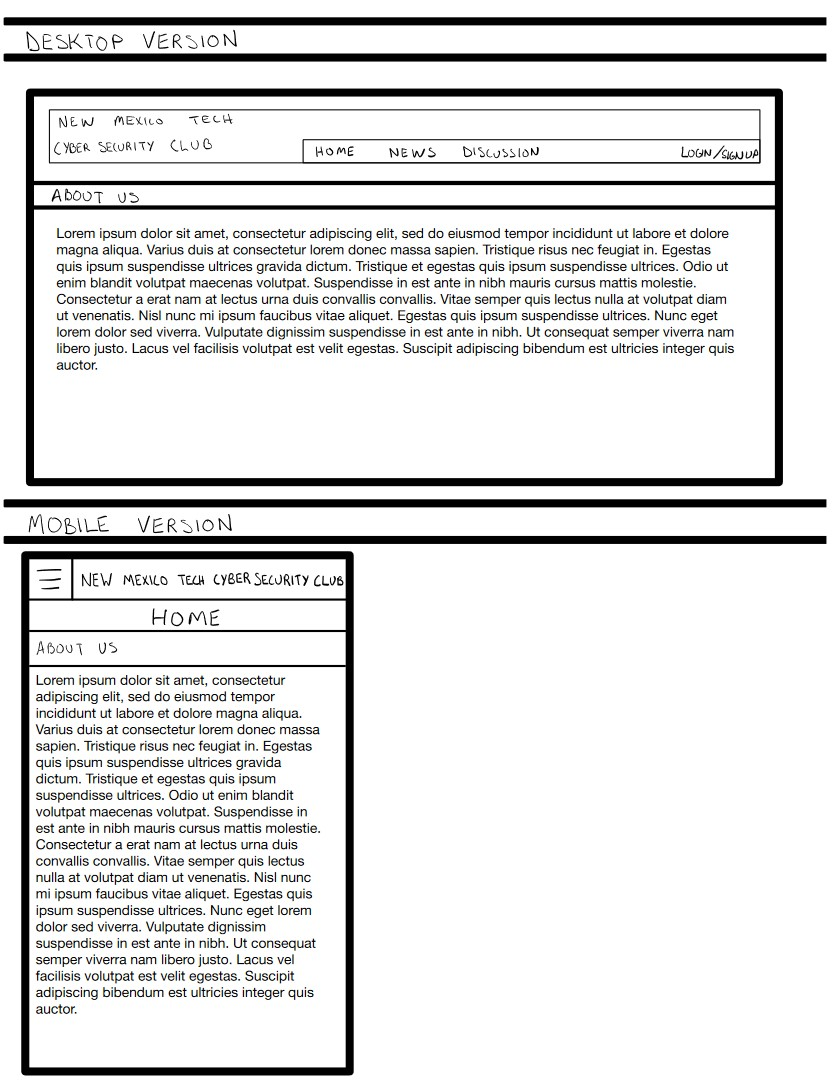
\includegraphics[scale=0.60]{visitor_1.jpg}
The Visitor then decides to check out the ‘News’ page.  They click on ‘News’ and then they are directed to a new page.  
\par
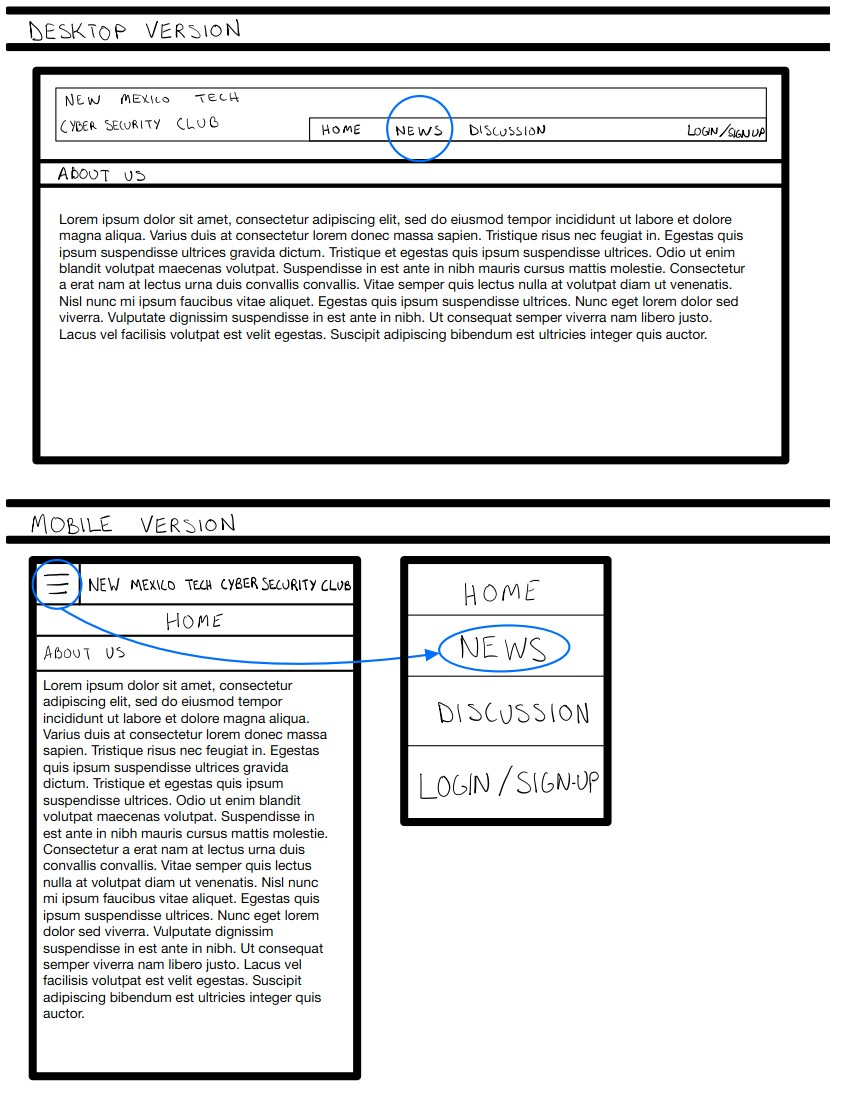
\includegraphics[scale=0.60]{visitor_2.jpg}
This new page simply replaces the ‘About Us’ section with posts related to relevant news articles under a new ‘News’ header, but also keeps everything from the ‘Home’ page the same.  The posts under the ‘News’ section contains: a title, brief description of the article, and tags or keywords found within the article.  If the Visitor or any other user decides to click on any of the posts, then they will be redirected to the source of the article on a new page.  The Visitor clicks on the first article and the source opens on their browser.
\par
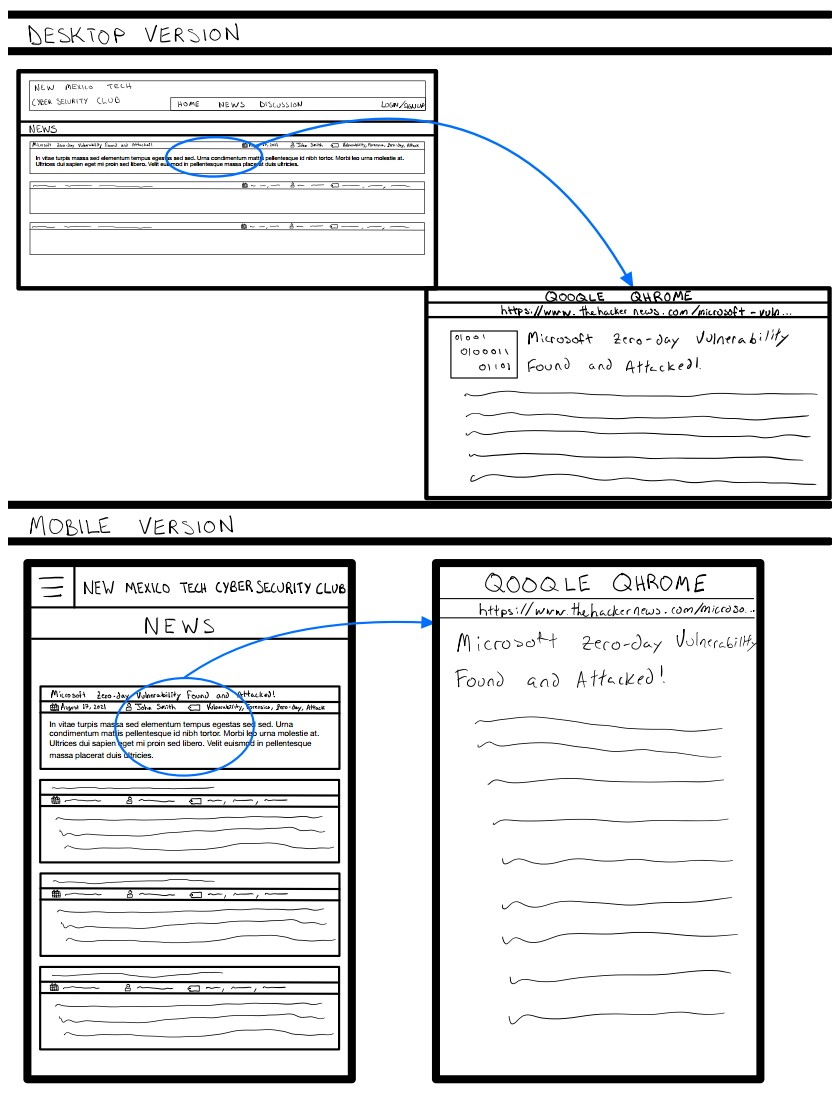
\includegraphics[scale=0.60]{visitor_3.jpg}
\par The Visitor then wishes to head on over to the ‘Discussion’ section.  They click on ‘Discussion’ and are redirected to the new page.  
\par
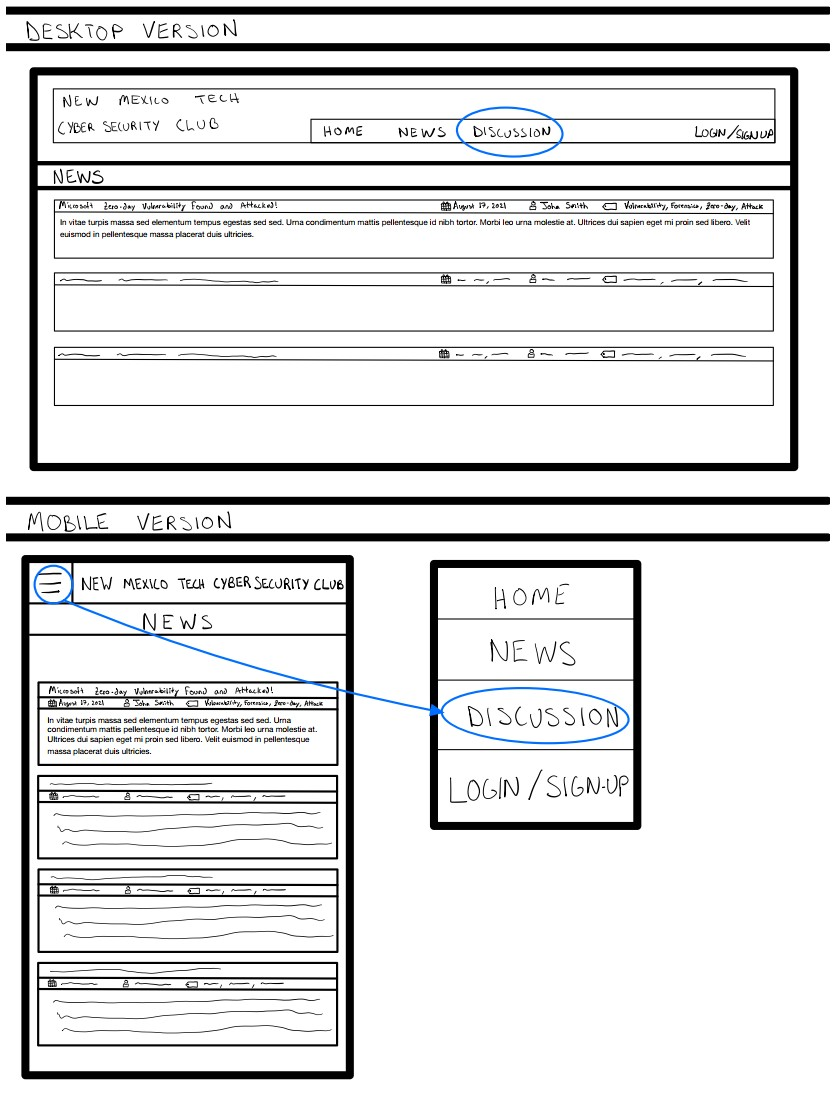
\includegraphics[scale=0.60]{visitor_4.jpg} 
\par Like the ‘News’ section, the layout is the similar with the title changed to ‘Discussion’ and various amounts of posts being discussed over.  The Visitor clicks on the first post and is shown the discussion board.
\par
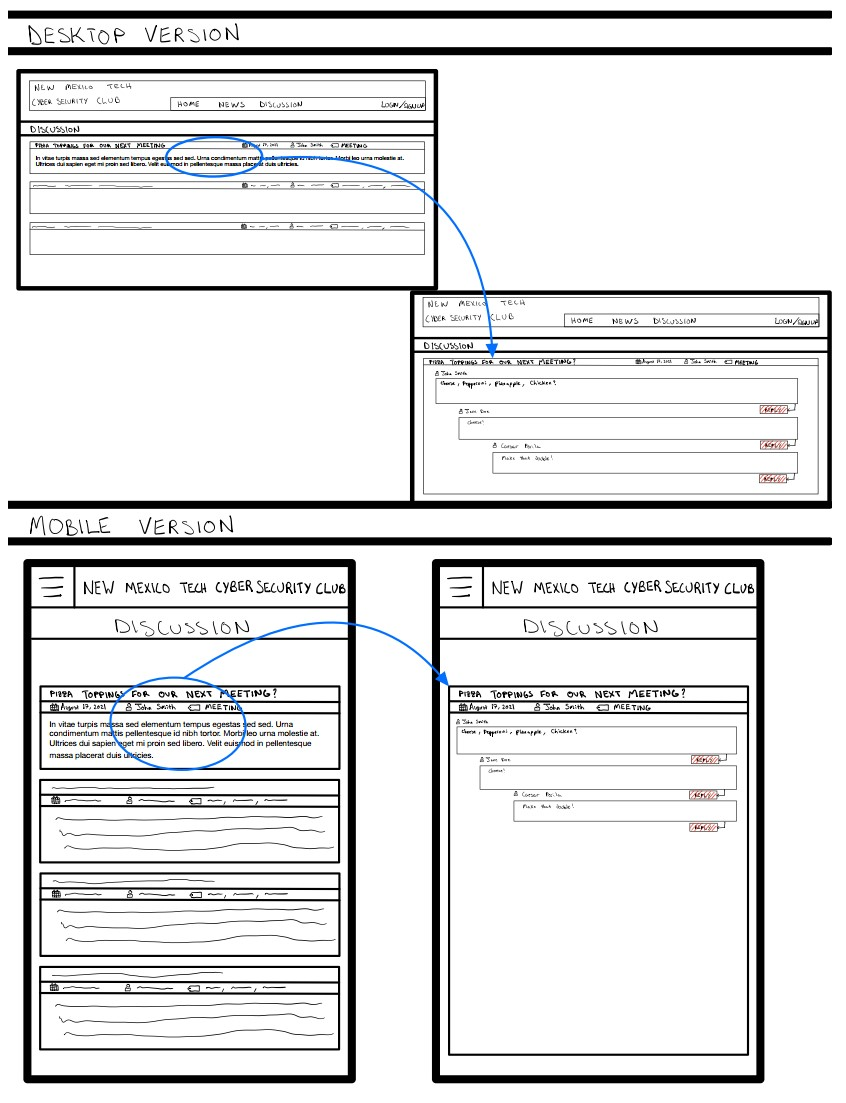
\includegraphics[scale=0.60]{visitor_5.jpg}
\par The post is having a discussion on what type of pizza toppings the club would like to have for their next meeting.  The Visitor sees various replies and notices that they themselves cannot reply for the button is grayed out.  They wish to partake in the pizza toppings discussion, so they decide they want to signup for the website.  They click the Log In/Signup button at the top-right of the page and are shown the Log In page.
\par
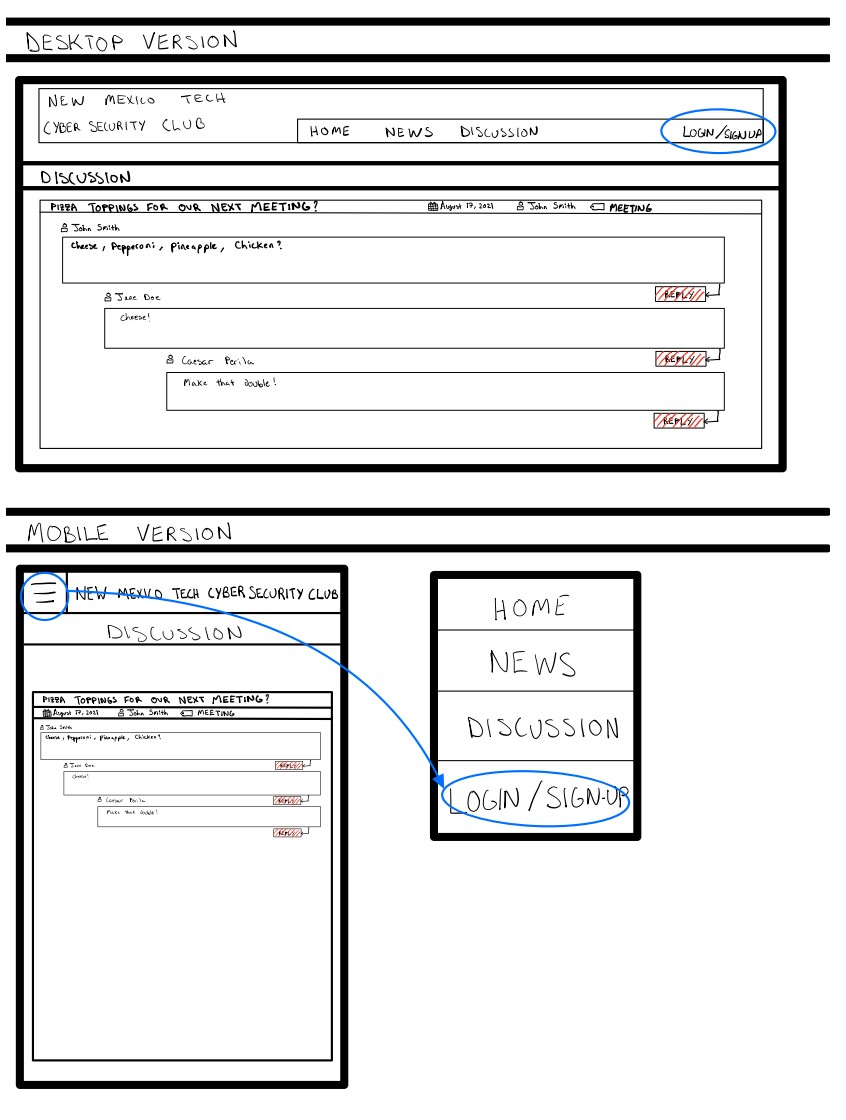
\includegraphics[scale=0.60]{visitor_6.jpg}
\par
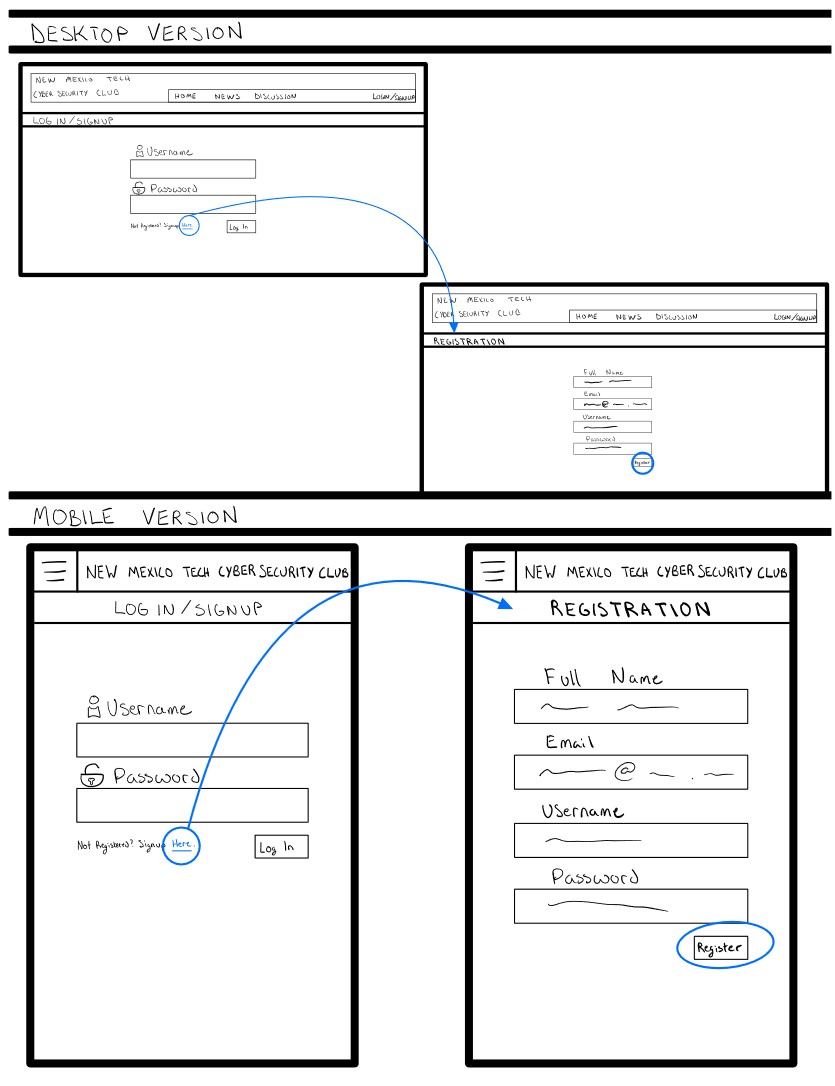
\includegraphics[scale=0.60]{visitor_7.jpg}
\par The Visitor clearly does not have a username or password yet, so they must register.  They click on ‘Here’ highlighted in blue and are redirected to the ‘Signup’ page.  They enter their information and now wait for approval from an officer of the club.

\par
\textbf{Club Member}: Around the same time, a ‘Member’ of the club recently saw a hot new controversial topic about cybersecurity and wants to share it on the discussion board.  They first click on the Log In/Signup link at the top right and are redirected to the log in page.  
\par
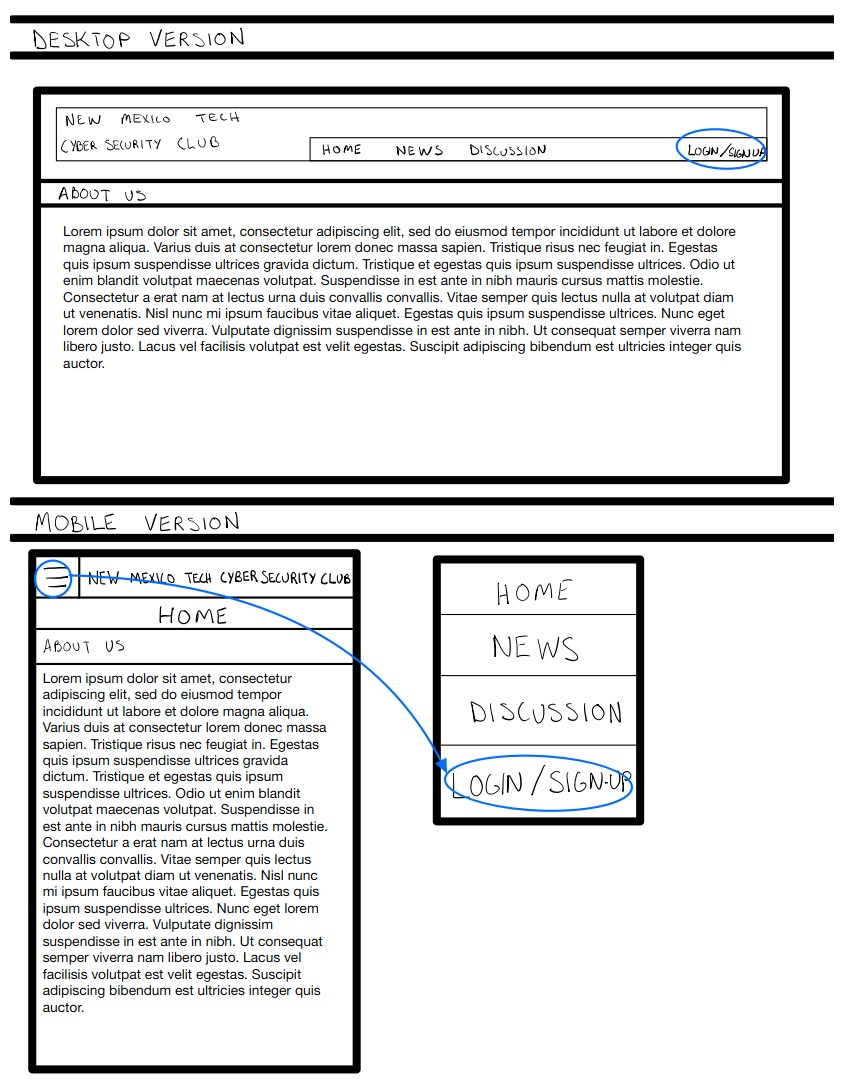
\includegraphics[scale=0.60]{member_1.jpg} They enter their information and are redirected back to the homepage. 
\par
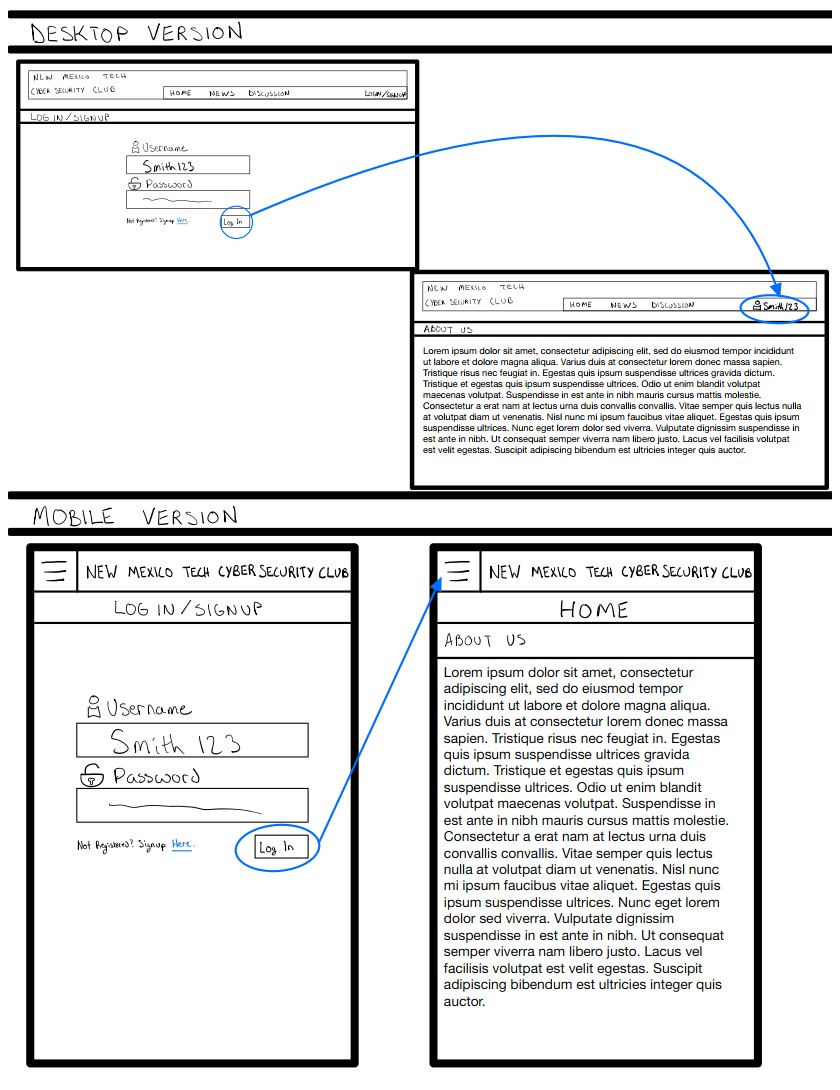
\includegraphics[scale=0.60]{member_2.jpg} The Member then clicks on Discussion and is shown the Discussion page but with a few more options than the Visitor.  The Member can click on a new button, ‘New Post’, allowing them to create a new post.  
 Upon clicking ‘New Post’ they are shown a new layout letting them write a title, a description, add any provided tags, and then confirm their post.  
\par
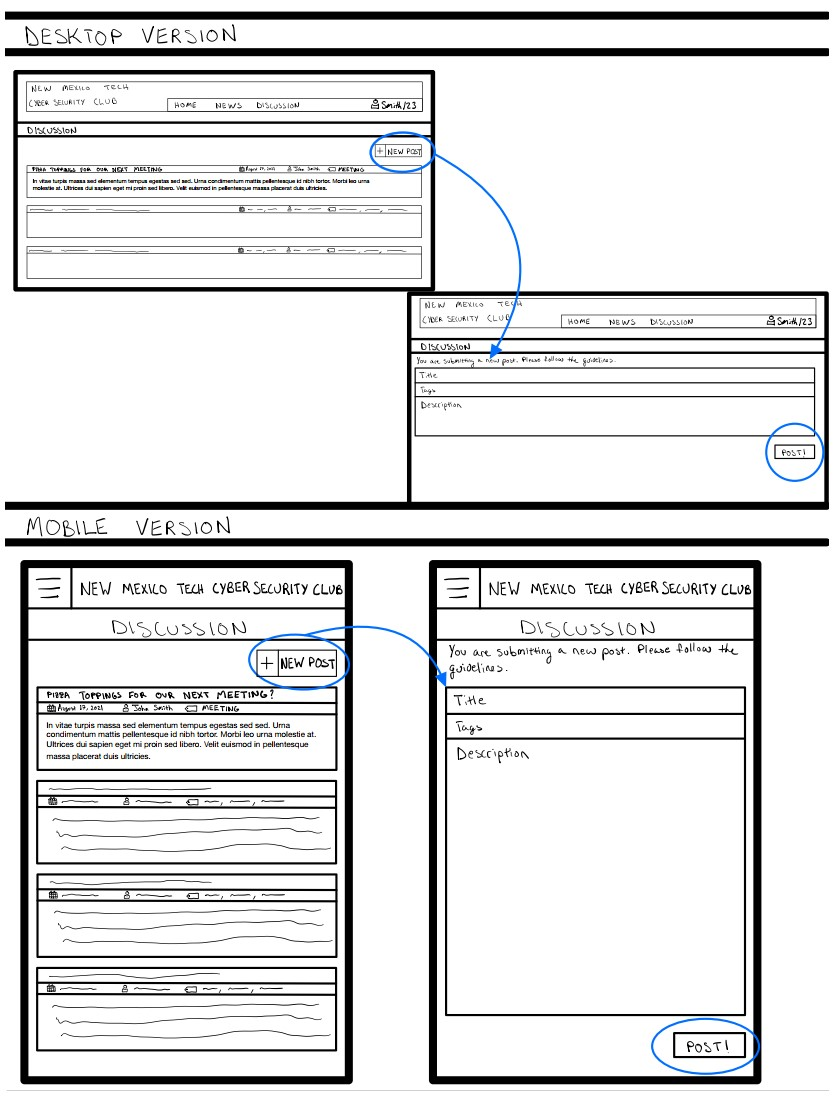
\includegraphics[scale=0.60]{member_3.jpg} The Member creates the new post and must wait for an Officer to to approve of the post. After creating the new post, the Member realizes they had an ongoing conversation from last night that they forgot to reply to.  They find the post and open it.  
\par
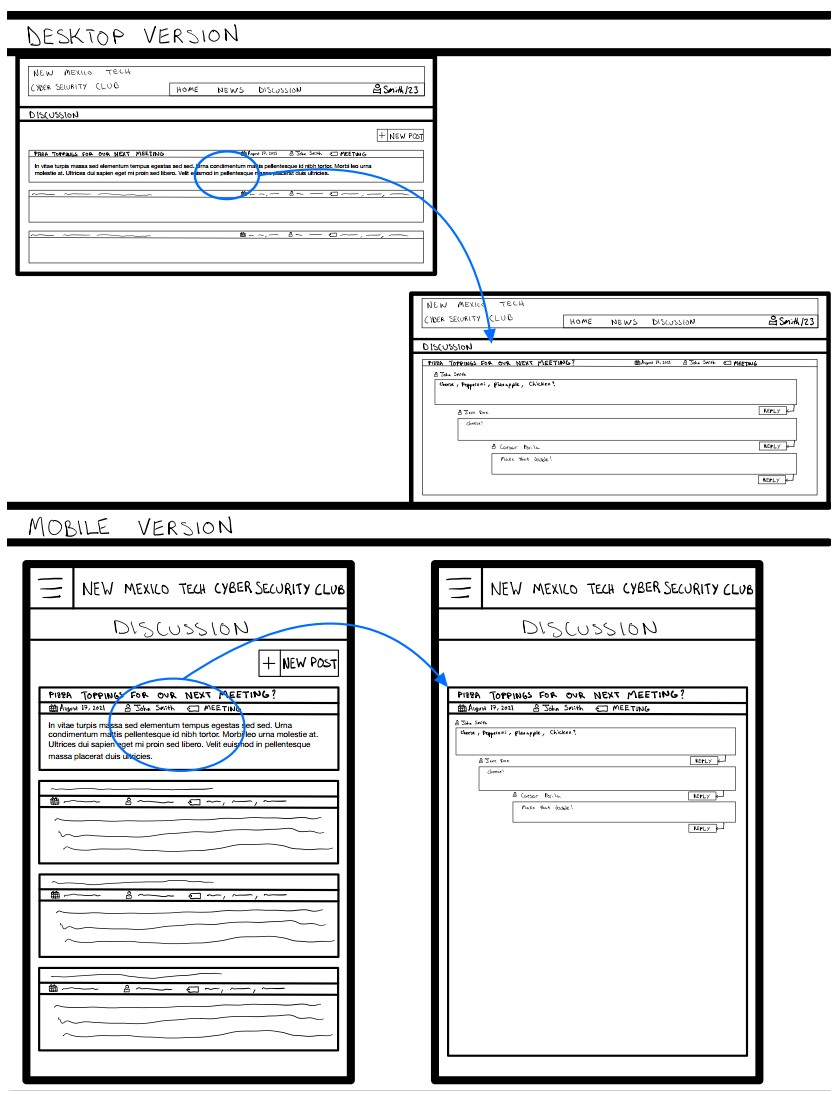
\includegraphics[scale=0.60]{member_4.jpg} They look up and down the post to see if any new posts were added.  A new post was indeed added and the Member decides to reply to it.  The ‘Reply’ button that was grayed out for the Visitor is visible and clickable for the Member.  The Member clicks on the button and enters a reply.  
\par
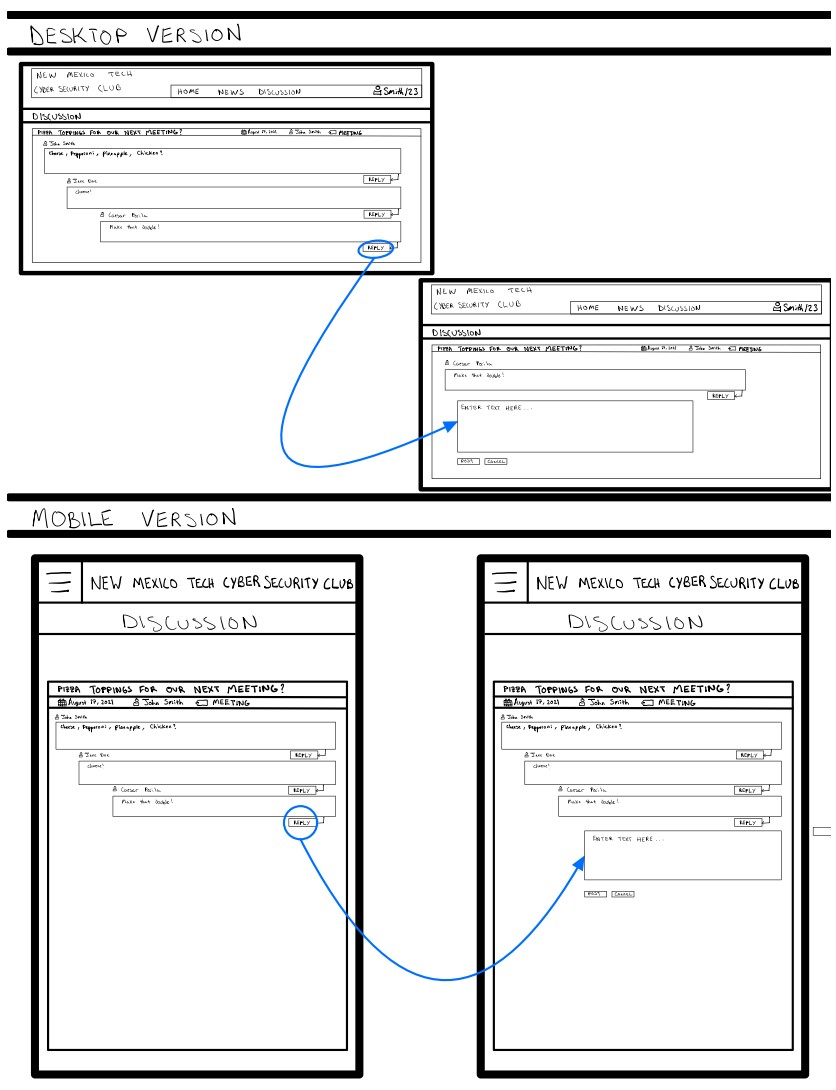
\includegraphics[scale=0.60]{member_5.jpg} It is their lunch time so they get up and leave for lunch at Chartwells.

\par
\textbf{Club Officers}: An officer of the club logs checks out the club website to see if there any new applications or posts to moderate.  They log in and are shown the homepage where there is a new menu option called 'Manage'. 
\par
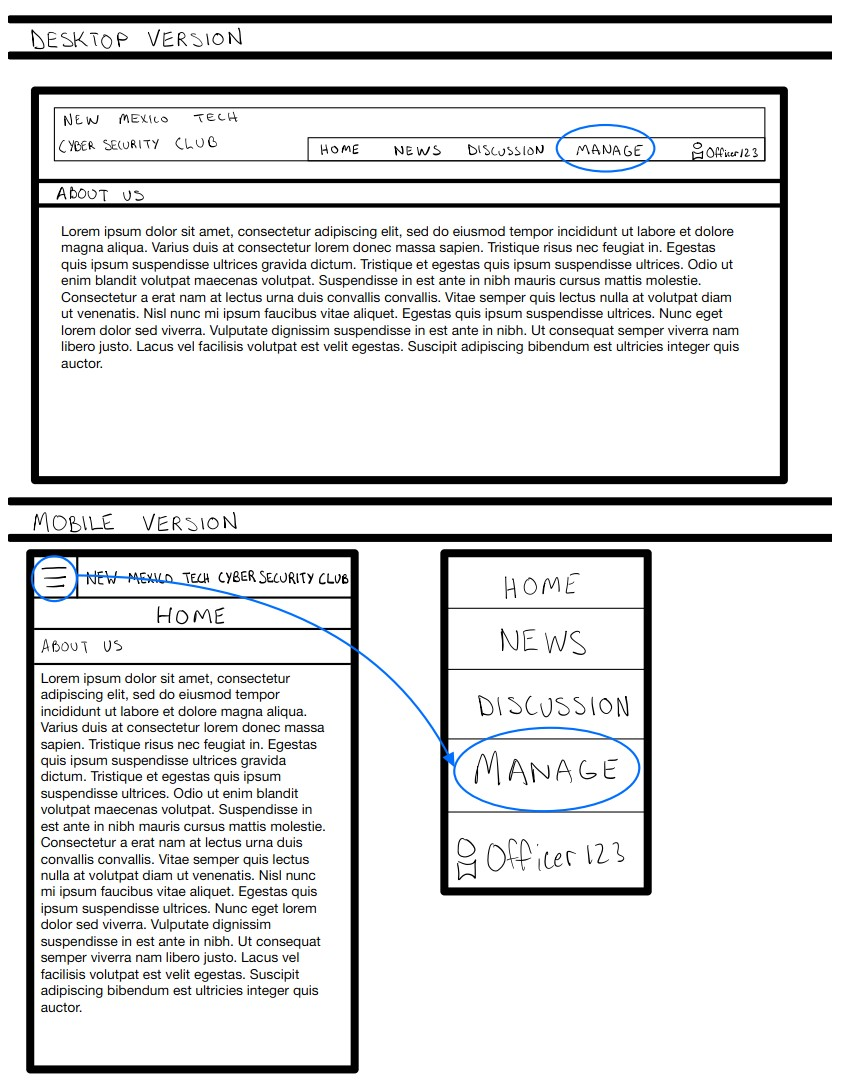
\includegraphics[scale=0.60]{officer_1.jpg} The Officer clicks on the 'Manage' tab and is redirected to the 'Manage' page.
\par
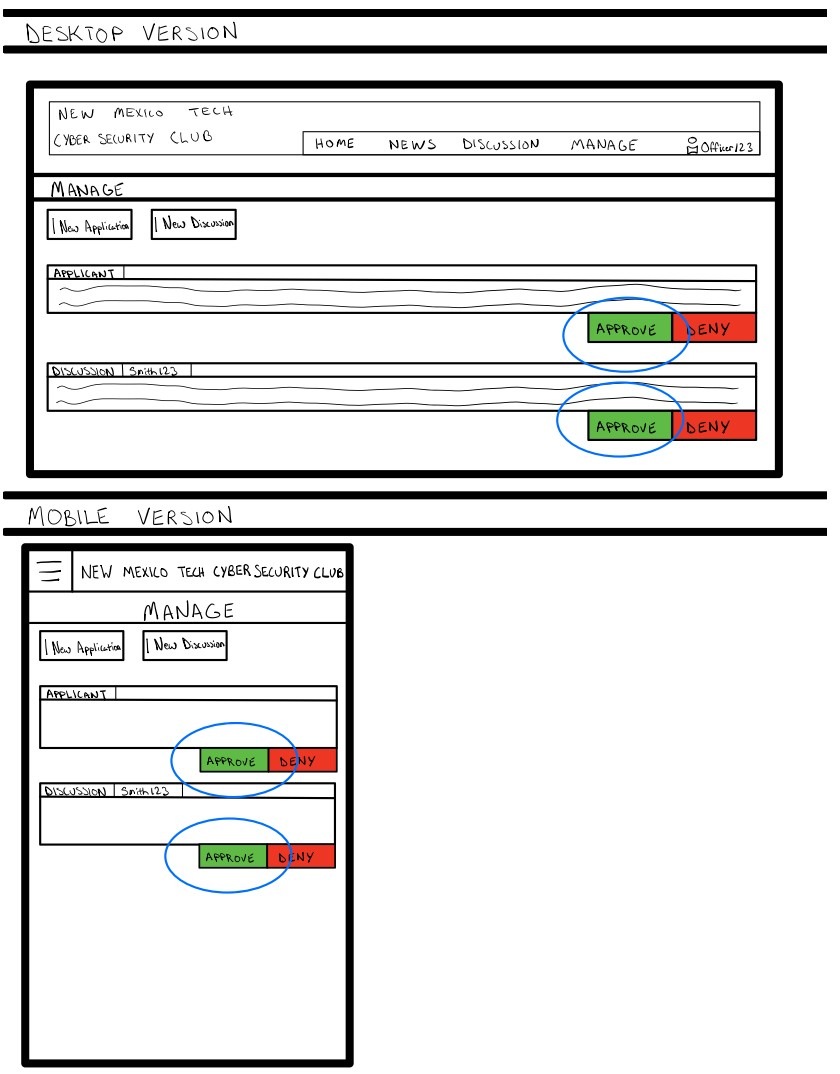
\includegraphics[scale=0.60]{officer_2.jpg} In the manage tab they notice two new notifications, one for a new applicant to the club website and the other for a new post in the discussion board.  The Officer reads over the application and the new discussion post and decides to approve both of them.  The Officer is done for the day for they must take a nap before their 3:00 p.m. math class.
 
  
  
\end{document}